\documentclass[aspectratio=169]{beamer}
\usetheme{Madrid}
\usepackage{tikz}
\usetikzlibrary{arrows.meta,positioning}
\setbeamertemplate{navigation symbols}{}
\setbeamerfont{block body}{size=\small}
\newcommand{\code}[1]{\texttt{\small #1}}

\title[QUDT in Acquirium]{Units the Acquirium Way}
\subtitle{QUDT normalization \& conversion -- ingest path, API, and the code}
\date{}

\begin{document}

\frame{\titlepage}

\begin{frame}{Outline}
  \tableofcontents
\end{frame}

% ==================================================================
\section{The big picture}

\begin{frame}{Where QUDT sits}
  Acquirium = RDF knowledge graph (Oxigraph) $+$ TimescaleDB time series,
  fronted by a FastAPI server.
  \begin{itemize}
    \item A stream's metadata lives in the graph: a point linked to a unit,
          quantity kind, medium, \dots
    \item \textbf{QUDT} is the canonical vocabulary for units and quantity
          kinds (\code{qudt.org/vocab/unit/*}).
    \item Sources speak \code{"mg/L"}, \code{"kg"}, \code{"gallon per
          minute"} -- not URIs.
  \end{itemize}
  \begin{block}{The job}
    Map messy unit text $\rightarrow$ a canonical QUDT URI, and know how to
    convert numerically between two such URIs.
  \end{block}
\end{frame}

\begin{frame}{Code map}
  \small
  \begin{tabular}{@{}p{0.46\textwidth}p{0.50\textwidth}@{}}
    \hline
    \textbf{Module} & \textbf{Role} \\ \hline
    \code{Server/manager.py} & orchestration: startup, indexes, endpoints'
        business logic \\
    \code{Server/app.py} & FastAPI routes \\
    \code{Storage/graph\_store.py} & Oxigraph store; \emph{verbatim} graph
        ingest \\
    \code{TextMatch/qudt\_store.py} & parse/cache/diff QUDT vocab \\
    \code{TextMatch/embedding\_matcher.py} & two-stage surface +
        embedding index \\
    \code{TextMatch/resolver.py} & \code{ConceptResolver} -- the pipeline \\
    \code{internals/qudt\_units.py} & \code{QUDTUnitConverter} -- exact
        resolve + math \\ \hline
  \end{tabular}
\end{frame}

\begin{frame}{Two separate concerns}
  \begin{columns}[T]
    \column{0.5\textwidth}
    \textbf{Normalization (resolution)}\\[2pt]
    text / symbol $\rightarrow$ canonical URI
    \begin{itemize}
      \item fuzzy, ranked, context-aware
      \item \code{ConceptResolver}
      \item \code{GET /resolve\_text}
    \end{itemize}
    \column{0.5\textwidth}
    \textbf{Conversion}\\[2pt]
    URI $+$ value $\rightarrow$ value
    \begin{itemize}
      \item deterministic arithmetic
      \item \code{QUDTUnitConverter}
      \item \code{/resolve\_unit},
            \code{/conversion\_factors}
    \end{itemize}
  \end{columns}
  \vspace{6pt}
  \begin{block}{Shared substrate}
    One lazily-loaded converter instance
    (\code{Manager.\_ensure\_qudt\_converter}); the resolver calls only its
    \emph{resolution} methods, never its conversion math.
  \end{block}
\end{frame}

% ==================================================================
\section{Ingest path}

\begin{frame}[fragile]{Ingest is verbatim}
  \begin{semiverbatim}\scriptsize
POST /insert_graph                       app.py:insert_graph
  -> Manager.insert_graph()              manager.py:683
     -> GraphStore.insert_graph()        graph_store.py:208
          incoming = Graph(); incoming.parse(data, fmt)
          for triple in incoming: main.add(triple)   # as-is
          refresh_union()                # rebuild union graph
  \end{semiverbatim}
  \begin{itemize}
    \item No unit rewriting at ingest. \code{qudt:hasUnit "mg/L"} is stored
          exactly as sent.
    \item The old \code{GraphStore.\_normalize\_unit} was \textbf{deleted} --
          it was dead code and would have mutated stored data.
  \end{itemize}
  \begin{block}{Why}
    Stored data stays faithful to the source; normalization is a
    resolution-time service, re-derivable and debuggable.
  \end{block}
\end{frame}

% ==================================================================
\section{Startup \& indexes}

\begin{frame}[fragile]{Startup: what \code{Manager.\_\_init\_\_} builds}
  \begin{semiverbatim}\scriptsize
self._graph_matcher = EmbeddingMatcher(cache=.../embedding_cache/graph)
self._qudt_matcher  = EmbeddingMatcher(cache=.../embedding_cache/qudt)
self._qudt_store    = QUDTStore(data_dir)
self._concept_resolver = ConceptResolver(
    graph_matcher, qudt_matcher,
    converter_provider = self._ensure_qudt_converter)
self._startup_graph_index()      # synchronous
self._startup_qudt_task()        # synchronous
  \end{semiverbatim}
  \begin{itemize}
    \item Model: \code{BAAI/bge-small-en-v1.5} (fastembed), vectors
          L2-normalized.
    \item \code{\_ensure\_qudt\_converter} lazily loads
          \code{QUDTUnitConverter("ontologies/qudt\_unit.ttl")}.
    \item Build state per index in \code{\_embedding\_status} ->
          \code{GET /embedding\_status}.
  \end{itemize}
\end{frame}

\begin{frame}[fragile]{Graph matcher: concepts from the data graph}
  \code{Manager.\_extract\_concepts\_for\_embedding()} runs four SPARQL
  extractions over the \emph{union} graph:
  \begin{semiverbatim}\scriptsize
class      : ?uri a rdfs:Class / owl:Class / ?x a ?uri / ...
predicate  : ?uri a rdf:Property / owl:*Property / ?s ?uri ?o
unit       : ?uri a qudt:Unit | ?x acq:hasUnit ?uri
quantity_kind: ?uri a qudt:QuantityKind | ?x acq:hasQuantityKind ?uri
  \end{semiverbatim}
  \begin{itemize}
    \item Unit/QK rows also surface \code{qudt:symbol} \&
          \code{qudt:ucumCode} so \code{"mg/l"}, \code{"kg"} embed well.
    \item \code{\_aggregate\_uri\_label\_rows} $\rightarrow$ concept dicts
          $\rightarrow$ \code{\_graph\_matcher.build\_index(concepts)}.
    \item Graph-defined units thus \emph{outrank} the broad QUDT vocab.
  \end{itemize}
\end{frame}

\begin{frame}[fragile]{QUDT matcher: \code{QUDTStore}}
  \begin{semiverbatim}\scriptsize
QUDTStore.extract_and_diff():
  _parse_ontology(QUDT_UNIT_url, ontologies/qudt_unit.ttl, qudt:Unit)
  _parse_ontology(QUDT_QK_url,   ontologies/qudt_qk.ttl,  qudt:QuantityKind)
  diff vs gzip cache  ->  (all_concepts, removed_uris, changed)
  save units.json.gz / qk.json.gz
  \end{semiverbatim}
  Per concept dict: \code{uri, kind, label, surfaces, symbol, ucum,
  related}.
  \begin{itemize}
    \item Surfaces = lower(labels) $+$ split-local-name $+$ symbol $+$ ucum.
    \item \code{related} = \code{qudt:hasQuantityKind} (units) /
          \code{qudt:applicableUnit} (QKs) -- powers context rerank.
    \item HTTP-first, local fallback; cache makes restarts incremental
          (\code{matcher.update\_index(added, removed)}).
  \end{itemize}
\end{frame}

% ==================================================================
\section{The matcher}

\begin{frame}[fragile]{\code{EmbeddingMatcher}: index \& two-stage query}
  \begin{semiverbatim}\scriptsize
build_index(concepts):
  hash -> _try_load_cache({hash}_vectors.npz/_meta.json)
  surfaces,meta = _build_surfaces_and_meta(concepts)
  vectors = _embed(surfaces)            # fastembed, L2-norm
  _set_index(vectors, meta, surface_index, surface_index_cs)

query(text, kind, top_k, min_score):
  1) _exact_stage : surface_index_cs (case) then casefold; score 1.0
  2) _semantic_stage: cosine = q_vec @ vectors.T ; kind mask ; cutoff
  -> [ResolveResult(uri,kind,label,score,matched_surface,
                    match_stage, related)]
  \end{semiverbatim}
  Exact-first because QUDT case matters: \code{kg} (kilogram) vs \code{kG}
  (kilogauss). Two surface maps (case-sensitive + casefold) keep both
  readings reachable.
\end{frame}

% ==================================================================
\section{ConceptResolver pipeline}

\begin{frame}[fragile]{\code{ConceptResolver.resolve} -- control flow}
  \begin{semiverbatim}\scriptsize
fetch_k = 20 if context else top_k        # over-fetch to rerank

if kind in (class, predicate):
    results = graph_matcher.query()
elif kind in (unit, quantity_kind):
    graph_hits = graph_matcher.query(min_score=0.8)
    if graph_hits and graph_hits[0].match_stage == "exact":
        results = graph_hits              # short-circuit
    else:
        det = _deterministic_unit(text) if kind=="unit" else []
        results = _combine(graph_hits + det, qudt_matcher.query())
else:
    results = _combine(graph_matcher.query(), qudt_matcher.query())

if context: results = _rerank_by_context(results, context)
return results[:top_k]
  \end{semiverbatim}
\end{frame}

\begin{frame}[fragile]{The deterministic unit tier}
  \code{ConceptResolver.\_deterministic\_unit(text)}:
  \begin{semiverbatim}\scriptsize
conv = converter_provider()               # _ensure_qudt_converter
try:    ud = conv.resolve_unit(text)
except UnitNotFound: ud = conv.infer_unit(text)
if str(ud.uri).startswith("urn:qudt:ratio:"): return []   # skip synth
return [ResolveResult(uri, kind="unit", score=1.0,
        match_stage="exact", related=ud.quantity_kinds)]
  \end{semiverbatim}
  \begin{itemize}
    \item Units only (mirrors the old client deterministic path).
    \item Authoritative: a hit is exact, score 1.0, and carries its
          quantity kinds as \code{related} so context still applies.
    \item Synthetic composed ratios are \emph{not} emitted -- the
          matchers handled those before, no regression.
    \item Provider raises if no QUDT graph $\Rightarrow$ silently degrade
          to matchers.
  \end{itemize}
\end{frame}

\begin{frame}[fragile]{Merge \& context rerank}
  \begin{semiverbatim}\scriptsize
_combine(primary, secondary, limit):
  sort by (match_stage=="exact", score) desc, primary first
  dedupe by uri, cap at limit          # graph/converter win ties

_rerank_by_context(results, context):
  connected = [r for r if set(context) & set(r.related)]
  rest      = [r for r if not ...]
  return connected + rest              # stable within groups
  \end{semiverbatim}
  \begin{block}{Safety property}
    A wrong / missing context URI fails to intersect any
    \code{r.related} $\Rightarrow$ ordering unchanged. Context can
    \emph{only help}, never inject a wrong answer.
  \end{block}
\end{frame}

\begin{frame}{Context disambiguation in action}
  Same surface \code{"kg"}, two QUDT units:
  \begin{itemize}
    \item \code{unit:KiloGM} -- \code{related} $\ni$ quantitykind/Mass
    \item \code{unit:KiloGAUSS} -- \code{related} $\ni$
          quantitykind/MagneticFluxDensity
  \end{itemize}
  \code{resolve\_text("kg", kind=unit, context=[.../Mass])}:
  \begin{enumerate}
    \item converter tier $\Rightarrow$ KiloGM exact (related = Mass\dots)
    \item QUDT matcher exact $\Rightarrow$ also KiloGAUSS
    \item rerank: KiloGM connected to \code{Mass} $\Rightarrow$ promoted
  \end{enumerate}
  Swap context to \code{.../MagneticFluxDensity} $\Rightarrow$ KiloGAUSS
  wins. No context $\Rightarrow$ \code{\_combine} order (KiloGM, stable).
\end{frame}

% ==================================================================
\section{Conversion \& API}

\begin{frame}[fragile]{\code{QUDTUnitConverter}: resolution ladder}
  \code{resolve\_unit(identifier)} -- first match wins:
  \begin{semiverbatim}\scriptsize
1 direct URIRef / http(s) URI
2 UNIT[identifier] / UNIT[UPPER] / UNIT[norm: space,hyphen->_]
3 COMMON_ALIASES  (gal->GAL_US, degc->DEG_C, ...)
4 literal == over [rdfs:label, skos:prefLabel,
    qudt:symbol, qudt:ucumCode, qudt:uneceCommonCode]
    case-sensitive, then casefold
else raise UnitNotFound
  \end{semiverbatim}
  \code{infer\_unit} adds: URI fragment/last-segment; ratio split
  (\code{" per "}, \code{"/"}) preferring a real \code{X-PER-Y} unit, else
  a synthetic \code{urn:qudt:ratio:} \code{\_compose\_ratio}; label
  substring search.
\end{frame}

\begin{frame}[fragile]{Conversion math}
  \code{UnitDefinition.from\_graph}: \code{conversionMultiplier},
  \code{conversionOffset}, quantity kind(s), dimension vector
  (\code{FIXED\_MULTIPLIERS} / \code{\_refine\_ratio\_multiplier} patch
  edge cases).
  \begin{block}{\code{convert(value, from, to)} -- Decimal, prec 28}
    \centering
    $K = (X + \text{offset}_{src})\cdot \text{mult}_{src}$ \quad(SI anchor)\\[2pt]
    $X' = K / \text{mult}_{tgt} - \text{offset}_{tgt}$
  \end{block}
  \code{\_check\_compatible}: dimension vector equality first, then
  quantity-kind overlap (raises \code{IncompatibleUnits} otherwise).
\end{frame}

\begin{frame}[fragile]{API surface}
  \small
  \begin{tabular}{@{}p{0.34\textwidth}p{0.58\textwidth}@{}}
    \hline
    \textbf{Endpoint $\rightarrow$ handler} & \textbf{Returns} \\ \hline
    \code{GET /resolve\_text}\newline
      \footnotesize\code{Manager.resolve\_text} &
      ranked \code{matches}: uri, kind, label, score, match\_stage,
      related (the pipeline; \code{asdict} of \code{ResolveResult}) \\[5pt]
    \code{POST /resolve\_unit}\newline
      \footnotesize\code{Manager.resolve\_unit\_info} &
      uri, label, symbol, quantity\_kind, multiplier, offset
      (converter direct) \\[5pt]
    \code{POST /conversion\_factors}\newline
      \footnotesize\code{Manager.get\_conversion\_factors} &
      src/tgt multipliers \& offsets $+$ \code{compatible} -- caller
      applies the arithmetic \\[5pt]
    \code{GET /embedding\_status} & per-index build state (graph, qudt) \\
    \hline
  \end{tabular}
  \vspace{4pt}\\
  \footnotesize
  Only \code{resolve\_text} goes through \code{ConceptResolver};
  conversion endpoints call \code{QUDTUnitConverter} directly.
\end{frame}

% ==================================================================
\section{End to end}

\begin{frame}{A unit string's journey}
  \centering
  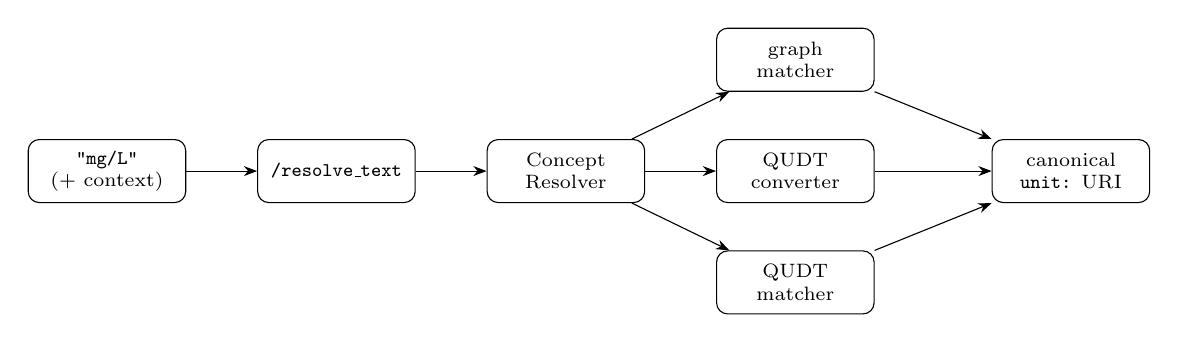
\begin{tikzpicture}[
      node distance=6mm and 9mm,
      box/.style={draw, rounded corners, align=center, font=\scriptsize,
                  minimum height=8mm, minimum width=20mm},
      >={Stealth[]}]
    \node[box] (in) {\texttt{"mg/L"}\\(+ context)};
    \node[box, right=of in] (api) {\texttt{/resolve\_text}};
    \node[box, right=of api] (res) {Concept\\Resolver};
    \node[box, above right=of res] (gx) {graph\\matcher};
    \node[box, right=of res] (cv) {QUDT\\converter};
    \node[box, below right=of res] (sem) {QUDT\\matcher};
    \node[box, right=44mm of res] (out) {canonical\\\texttt{unit:} URI};
    \draw[->] (in) -- (api);
    \draw[->] (api) -- (res);
    \draw[->] (res) -- (gx);
    \draw[->] (res) -- (cv);
    \draw[->] (res) -- (sem);
    \draw[->] (gx) -- (out);
    \draw[->] (cv) -- (out);
    \draw[->] (sem) -- (out);
  \end{tikzpicture}
  \vspace{4pt}

  \footnotesize
  Tiers tried in order; \code{\_combine} merges (exact-first), then
  \code{\_rerank\_by\_context}. The stored graph is never touched.
\end{frame}

\begin{frame}{Takeaways}
  \begin{itemize}
    \item Ingest is faithful; normalization is a service, not a mutation.
    \item One server-side \code{ConceptResolver} = data graph $+$
          deterministic converter $+$ QUDT embeddings $+$ context.
    \item Resolution and conversion are deliberately separate code paths
          sharing one converter instance.
    \item Exact-first everywhere; context can only help; everything
          re-derivable from the graph $+$ QUDT vocab.
  \end{itemize}
\end{frame}

\end{document}
